\documentclass[border=0pt]{standalone}
\usepackage[T1]{fontenc}
\usepackage[utf8]{inputenc}
\usepackage{helvet}
\usepackage{amsmath}
\usepackage{tikz}
\renewcommand{\familydefault}{\sfdefault}
\usetikzlibrary{arrows.meta,calc,positioning,shadings}

% Step 1 design note for thesis-figure-skill.
% Complex five-zone horizontal framework, W x H = 14.91 x 10.55 logical cm.
% Visual flow: fixed inputs -> controls -> lower-level simulator -> performance -> optimizer.
% The simulator is the hero zone: it embeds stage blocks, formula cues, and output mini-viz.
% Polish targets: aligned headers, bounded text, uniform math/text scale, and readable feedback loop.

\definecolor{navy}{RGB}{0,57,122}
\definecolor{blue}{RGB}{20,98,181}
\definecolor{lineblue}{RGB}{0,57,122}
\definecolor{lightblue}{RGB}{238,247,255}
\definecolor{pale}{RGB}{248,252,255}

\tikzset{
  panel/.style={rounded corners=0.08cm, draw=lineblue, line width=0.018cm, fill=white},
  header/.style={rounded corners=0.08cm, draw=lineblue, line width=0.018cm, fill=navy},
  box/.style={rounded corners=0.07cm, draw=blue, line width=0.014cm, fill=white},
  smallbox/.style={rounded corners=0.06cm, draw=blue, line width=0.011cm, fill=white},
  titletext/.style={font=\bfseries\fontsize{10.8}{12.4}\selectfont, text=black, align=center},
  headtext/.style={font=\bfseries\fontsize{5.35}{6.2}\selectfont, text=white, align=center, execute at begin node={\everymath{\scriptstyle}}},
  bodytext/.style={font=\bfseries\fontsize{4.25}{5.15}\selectfont, text=black, align=left, execute at begin node={\everymath{\scriptstyle}}},
  smalltext/.style={font=\fontsize{3.45}{4.15}\selectfont, text=black, align=left, execute at begin node={\everymath{\scriptscriptstyle}}},
  tinytext/.style={font=\fontsize{3.25}{3.90}\selectfont, text=black, align=left, execute at begin node={\everymath{\scriptscriptstyle}}},
  labelblue/.style={font=\bfseries\fontsize{4.85}{5.65}\selectfont, text=navy, align=center, execute at begin node={\everymath{\scriptstyle}}},
  arrow/.style={-{Stealth[length=0.18cm,width=0.20cm]}, line width=0.045cm, draw=black},
  flowarrow/.style={-{Stealth[length=0.13cm,width=0.15cm]}, line width=0.018cm, draw=lineblue},
  downflow/.style={-{Stealth[length=0.070cm,width=0.085cm]}, line width=0.014cm, draw=lineblue},
}

\tikzset{
  gridicon/.pic={
    \draw[blue, line width=0.012cm] (-0.22,-0.22) rectangle (0.22,0.22);
    \foreach \x in {-0.11,0,0.11}{\draw[blue!70,line width=0.006cm] (\x,-0.22)--(\x,0.22);}
    \foreach \y in {-0.11,0,0.11}{\draw[blue!70,line width=0.006cm] (-0.22,\y)--(0.22,\y);}
  },
  curveicon/.pic={
    \draw[blue,line width=0.012cm] (-0.24,-0.18)--(-0.24,0.22);
    \draw[blue,line width=0.012cm] (-0.24,-0.18)--(0.24,-0.18);
    \draw[lineblue,line width=0.018cm] plot[smooth] coordinates {(-0.20,-0.12) (-0.08,-0.04) (0.02,0.12) (0.12,0.00) (0.22,0.08)};
  },
  diricon/.pic={
    \draw[flowarrow] (0,0)--(0,0.25);
    \draw[flowarrow] (0,0)--(0,-0.25);
    \draw[flowarrow] (0,0)--(0.26,0);
    \draw[lineblue,line width=0.012cm] (-0.18,0.16) .. controls (-0.09,0.05) and (-0.07,-0.04) .. (-0.16,-0.16);
  },
  contouricon/.pic={
    \foreach \r in {0.08,0.15,0.22}{
      \draw[blue,line width=0.010cm] (0,0) ellipse ({1.18*\r} and {\r});
    }
    \draw[blue,line width=0.010cm, rotate=28] (0,0) ellipse (0.27 and 0.19);
  },
  cubeicon/.pic={
    \draw[blue,line width=0.012cm] (-0.12,-0.18)--(0.08,-0.08)--(0.08,0.15)--(-0.12,0.25)--cycle;
    \draw[blue,line width=0.012cm] (0.08,-0.08)--(0.25,0.03)--(0.25,0.25)--(0.08,0.15)--cycle;
    \draw[blue,line width=0.012cm] (-0.12,0.25)--(0.05,0.35)--(0.25,0.25);
    \draw[blue,line width=0.012cm] (0.05,0.35)--(0.08,0.15);
  },
  gateicon/.pic={
    \draw[blue,line width=0.012cm] (-0.22,-0.22) rectangle (0.07,0.24);
    \draw[blue,line width=0.012cm] (-0.17,-0.22)--(-0.17,0.17)--(0.02,0.17)--(0.02,-0.22);
    \fill[navy] (-0.10,-0.03) circle (0.045);
    \draw[navy,line width=0.018cm] (-0.10,-0.08)--(-0.10,-0.19);
    \draw[flowarrow] (0.10,-0.05)--(0.30,-0.05);
  },
  spliticon/.pic={
    \draw[flowarrow] (-0.20,-0.18).. controls (-0.10,0.00) and (-0.08,0.04)..(0,0.04);
    \draw[flowarrow] (0,0.04).. controls (0.10,0.10) and (0.15,0.22)..(0.24,0.25);
    \draw[flowarrow] (0,0.04).. controls (0.10,0.02) and (0.17,-0.10)..(0.25,-0.16);
  },
  heaticon/.pic={
    \shade[inner color=yellow, outer color=blue!75] (-0.02,0.02) circle (0.30);
    \shade[inner color=orange, outer color=yellow!30] (-0.08,-0.02) circle (0.17);
    \shade[inner color=red!75, outer color=orange!40] (0.08,0.09) circle (0.13);
  },
  velocityicon/.pic={
    \foreach \y in {-0.16,0,0.16}{
      \foreach \x in {-0.18,0.03}{
        \draw[flowarrow] (\x,\y)--(\x+0.16,\y);
      }
    }
  },
  peopleicon/.pic={
    \fill[navy] (-0.16,0.13) circle (0.045);
    \draw[navy,line width=0.018cm] (-0.16,0.08)--(-0.16,-0.16);
    \draw[navy,line width=0.014cm] (-0.24,-0.02)--(-0.08,-0.02);
    \draw[navy,line width=0.014cm] (-0.20,-0.16)--(-0.20,-0.26);
    \draw[navy,line width=0.014cm] (-0.12,-0.16)--(-0.12,-0.26);
    \fill[navy] (0.13,0.08) circle (0.040);
    \draw[navy,line width=0.016cm] (0.13,0.03)--(0.13,-0.16);
    \draw[navy,line width=0.013cm] (0.06,-0.04)--(0.20,-0.04);
  },
  barsicon/.pic={
    \fill[navy!85] (-0.23,-0.23) rectangle (-0.14,0.05);
    \fill[navy!85] (-0.08,-0.23) rectangle (0.01,0.22);
    \fill[navy!85] (0.07,-0.23) rectangle (0.16,-0.02);
    \fill[navy!85] (0.22,-0.23) rectangle (0.31,0.13);
    \draw[blue,line width=0.010cm] (-0.28,-0.23)--(0.34,-0.23);
  }
}

\newcommand{\PanelWithHeader}[6]{%
  \draw[panel] (#1,#2) rectangle ++(#3,#4);
  \draw[header] (#1,#2+#4-#5) rectangle ++(#3,#5);
  \node[headtext, text width=#3 cm] at (#1+#3/2,#2+#4-#5/2) {#6};
}
\newcommand{\BoxAnchors}[5]{%
  \coordinate (#1-sw) at (#2,#3);
  \coordinate (#1-se) at (#2+#4,#3);
  \coordinate (#1-nw) at (#2,#3+#5);
  \coordinate (#1-ne) at (#2+#4,#3+#5);
  \coordinate (#1-west) at (#2,#3+#5/2);
  \coordinate (#1-east) at (#2+#4,#3+#5/2);
  \coordinate (#1-south) at (#2+#4/2,#3);
  \coordinate (#1-north) at (#2+#4/2,#3+#5);
  \coordinate (#1-center) at (#2+#4/2,#3+#5/2);
}
\newcommand{\PanelWithHeaderNamed}[7]{%
  \PanelWithHeader{#2}{#3}{#4}{#5}{#6}{#7}
  \BoxAnchors{#1}{#2}{#3}{#4}{#5}
}
\newcommand{\PanelWithHeaderNamedStyled}[8]{%
  \draw[panel,#8] (#2,#3) rectangle ++(#4,#5);
  \draw[header] (#2,#3+#5-#6) rectangle ++(#4,#6);
  \node[headtext, text width=#4 cm] at (#2+#4/2,#3+#5-#6/2) {#7};
  \BoxAnchors{#1}{#2}{#3}{#4}{#5}
}
\newcommand{\PanelHeaderOnly}[6]{%
  \draw[header] (#1,#2+#4-#5) rectangle ++(#3,#5);
  \node[headtext, text width=#3 cm] at (#1+#3/2,#2+#4-#5/2) {#6};
}
\newcommand{\SmallBox}[4]{\draw[box] (#1,#2) rectangle ++(#3,#4);}
\newcommand{\SmallBoxNamed}[5]{%
  \SmallBox{#2}{#3}{#4}{#5}
  \BoxAnchors{#1}{#2}{#3}{#4}{#5}
}
\newcommand{\TextBox}[6]{%
  \draw[box] (#1,#2) rectangle ++(#3,#4);
  \node[bodytext, anchor=north west, text width=#5 cm, align=left]
    at (#1+0.12,#2+#4-0.12) {#6};
}
\newcommand{\StageBox}[6]{%
  \draw[smallbox] (#1,#2) rectangle ++(#3,#4);
  \node[tinytext, anchor=north west, text width=#5 cm, align=left]
    at (#1+0.08,#2+#4-0.07) {#6};
}
\newcommand{\StageBoxNamed}[7]{%
  \StageBox{#2}{#3}{#4}{#5}{#6}{#7}
  \BoxAnchors{#1}{#2}{#3}{#4}{#5}
}
\newcommand{\OutputBox}[6]{%
  \draw[smallbox] (#1,#2) rectangle ++(#3,#4);
  \node[smalltext, anchor=west, text width=#5 cm, align=left]
    at (#1+0.08,#2+#4/2) {#6};
}
\newcommand{\Bullet}[3]{%
  \fill[black] (#1,#2) circle (0.043);
  \node[bodytext, anchor=west, text width=#3 cm] at (#1+0.03,#2)
}
\newcommand{\StepBox}[5]{%
  \draw[box] (#1,#2) rectangle ++(2.02,0.76);
  \fill[navy] (#1+0.23,#2+0.38) circle (0.14);
  \node[font=\bfseries\fontsize{6.2}{7.0}\selectfont, text=white] at (#1+0.23,#2+0.38) {#3};
  \node[bodytext, anchor=west, text width=2.30cm, align=left] at (#1+0.3,#2+0.39) {#4};
}
\newcommand{\StepBoxNamed}[5]{%
  \StepBox{#2}{#3}{#4}{#5}{}
  \BoxAnchors{#1}{#2}{#3}{1.82}{0.76}
}

\begin{document}
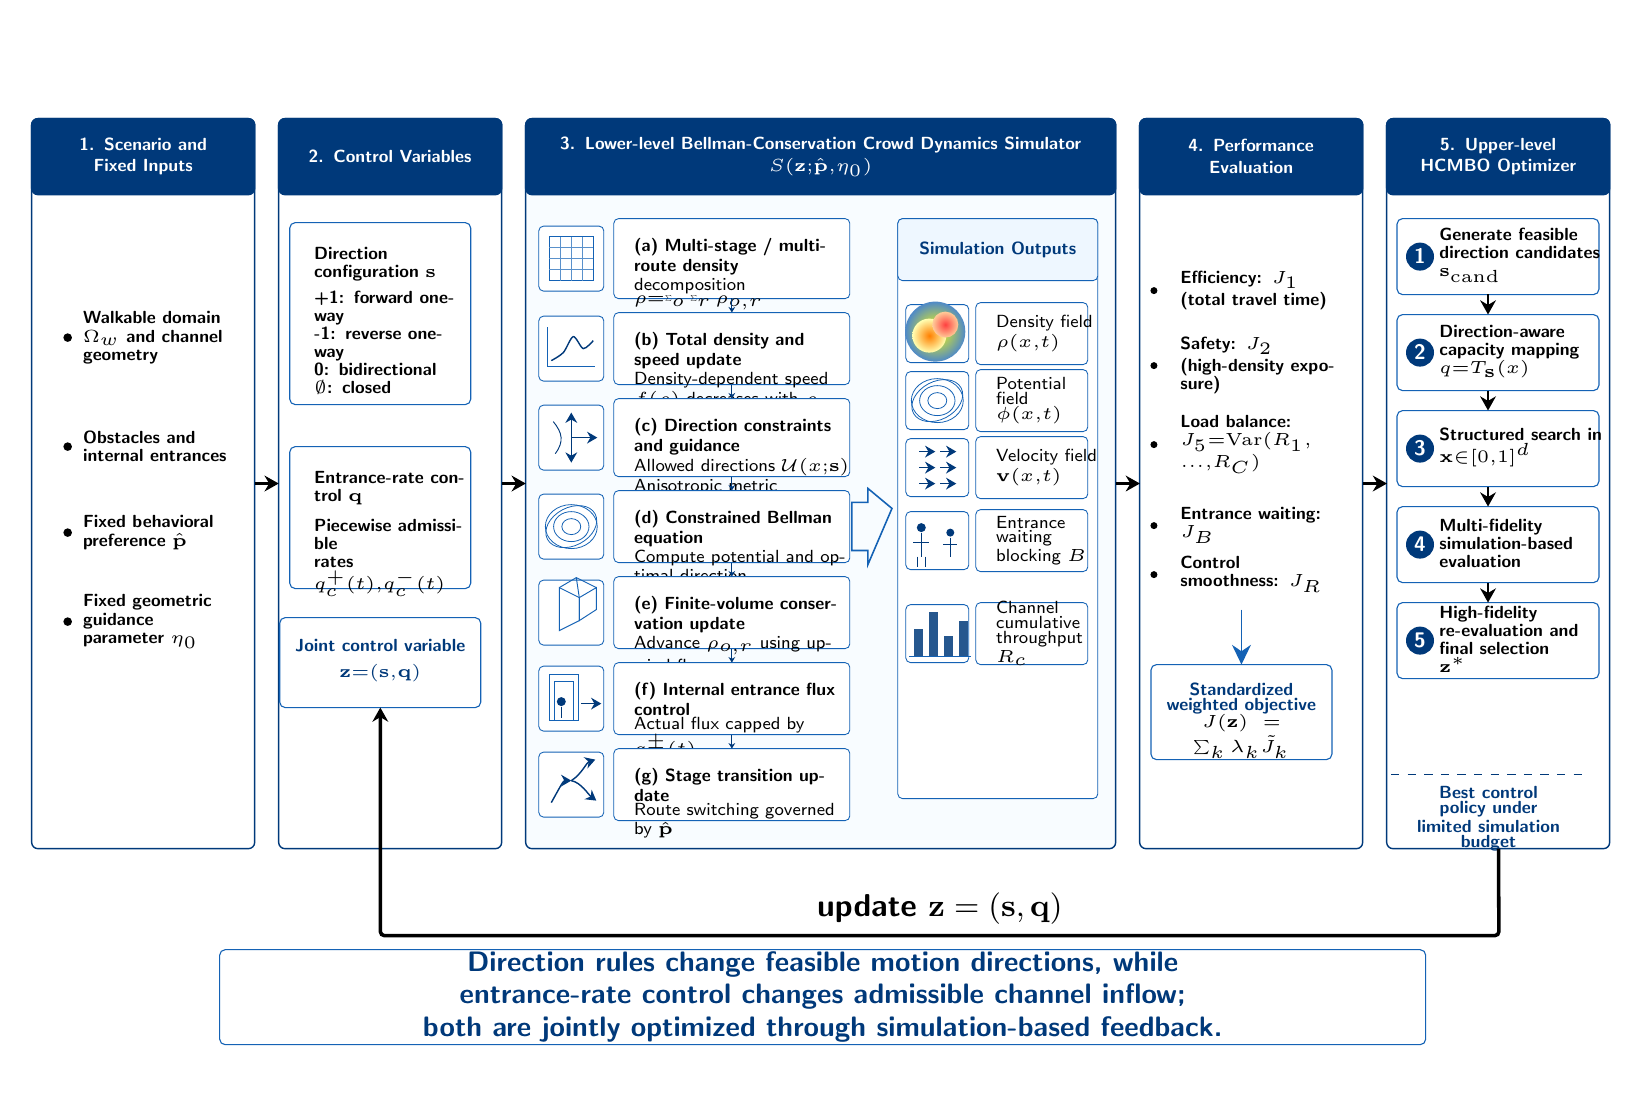
\begin{tikzpicture}[scale=1.27, transform shape]
  \def\sideW{2.23}
  \def\simW{5.90}
  \def\mainGap{0.24}
  \def\mainY{2.34}
  \def\mainH{7.30}
  \pgfmathsetmacro{\colOneX}{0.04}
  \pgfmathsetmacro{\colTwoX}{\colOneX+\sideW+\mainGap}
  \pgfmathsetmacro{\simX}{\colTwoX+\sideW+\mainGap}
  \pgfmathsetmacro{\colFourX}{\simX+\simW+\mainGap}
  \pgfmathsetmacro{\colFiveX}{\colFourX+\sideW+\mainGap}
  \pgfmathsetmacro{\canvasW}{\colFiveX+\sideW+0.08}
  \pgfmathsetmacro{\figCenter}{\canvasW/2}
  \pgfmathsetmacro{\bottomX}{\figCenter-6.03}

  \path[use as bounding box] (0,0) rectangle (\canvasW,10.55);
  \fill[white] (0,0) rectangle (\canvasW,10.55);

%  \node[titletext] at (\figCenter,10.18) {Method Framework for Joint Direction and Entrance-Rate Optimization};

  % Column 1
  \PanelWithHeaderNamed{col1}{\colOneX}{\mainY}{\sideW}{\mainH}{0.76}{1. Scenario and\\Fixed Inputs}
  \begin{scope}[shift={(col1-sw)}]
    \Bullet{0.36}{5.11}{1.45}{Walkable domain\\$\Omega_w$ and channel\\geometry};
    \Bullet{0.36}{4.02}{1.45}{Obstacles and\\internal entrances};
    \Bullet{0.36}{3.16}{1.45}{Fixed behavioral\\preference $\hat{\mathbf{p}}$};
    \Bullet{0.36}{2.27}{1.45}{Fixed geometric\\guidance\\parameter $\eta_0$};
  \end{scope}

  % Column 2
  \PanelWithHeaderNamed{col2}{\colTwoX}{\mainY}{\sideW}{\mainH}{0.76}{2. Control Variables}
  \begin{scope}[shift={(col2-sw)}]
    \TextBox{0.11}{4.44}{1.81}{1.82}{1.53}
      {\textbf{Direction\\configuration $\mathbf{s}$}\\[0.08cm]
      +1: forward one-way\\
      -1: reverse one-way\\
      0: bidirectional\\
      $\emptyset$: closed};
    \TextBox{0.11}{2.60}{1.81}{1.42}{1.53}
      {\textbf{Entrance-rate control $\mathbf{q}$}\\[0.12cm]
      Piecewise admissible\\rates $q_c^+(t), q_c^-(t)$};
    \SmallBoxNamed{joint-control}{0.01}{1.41}{2.01}{0.90}
    \node[labelblue, text width=1.76cm] at (1.015,1.88) {Joint control variable\\[0.06cm]$\mathbf{z}=(\mathbf{s},\mathbf{q})$};
  \end{scope}

  % Column 3 main simulator
  \PanelWithHeaderNamedStyled{sim-panel}{\simX}{\mainY}{\simW}{\mainH}{0.76}
    {3. Lower-level Bellman-Conservation Crowd Dynamics Simulator\\$S(\mathbf{z};\hat{\mathbf{p}},\eta_0)$}{fill=pale}
  \begin{scope}[shift={(sim-panel-sw)}]
    \def\ix{0.13}
    \def\iw{0.65}
    \def\tw{2.36}
    \def\tx{0.88}
    \foreach \y/\picname in {5.575/gridicon,4.675/curveicon,3.785/diricon,2.895/contouricon,2.035/cubeicon,1.175/gateicon,0.315/spliticon}{
      \draw[smallbox] (\ix,\y) rectangle ++(\iw,0.65);
      \pic at (\ix+0.325,\y+0.325) {\picname};
    }

    \StageBoxNamed{stage-a}{\tx}{5.50}{2.36}{0.80}{2.18}
      {\textbf{(a) Multi-stage / multi-route density}\\
       decomposition\\[-0.01cm]
       $\rho=\sum_o\sum_r\rho_{o,r}$};
    \StageBoxNamed{stage-b}{\tx}{4.64}{2.36}{0.72}{2.18}
      {\textbf{(b) Total density and speed update}\\
       Density-dependent speed\\
       $f(\rho)$ decreases with $\rho$};
    \StageBoxNamed{stage-c}{\tx}{3.72}{2.36}{0.78}{2.18}
      {\textbf{(c) Direction constraints and guidance}\\
       Allowed directions $\mathcal{U}(x;\mathbf{s})$\\
       Anisotropic metric $M(x;\eta_0)$};
    \StageBoxNamed{stage-d}{\tx}{2.86}{2.36}{0.72}{2.18}
      {\textbf{(d) Constrained Bellman equation}\\
       Compute potential and optimal direction};
    \StageBoxNamed{stage-e}{\tx}{2.00}{2.36}{0.72}{2.18}
      {\textbf{(e) Finite-volume conservation update}\\
       Advance $\rho_{o,r}$ using upwind fluxes};
    \StageBoxNamed{stage-f}{\tx}{1.14}{2.36}{0.72}{2.18}
      {\textbf{(f) Internal entrance flux control}\\
       Actual flux capped by $q_c^\pm(t)$};
    \StageBoxNamed{stage-g}{\tx}{0.28}{2.36}{0.72}{2.18}
      {\textbf{(g) Stage transition update}\\
       Route switching governed by $\hat{\mathbf{p}}$};

    \draw[downflow] (stage-a-south)--(stage-b-north);
    \draw[downflow] (stage-b-south)--(stage-c-north);
    \draw[downflow] (stage-c-south)--(stage-d-north);
    \draw[downflow] (stage-d-south)--(stage-e-north);
    \draw[downflow] (stage-e-south)--(stage-f-north);
    \draw[downflow] (stage-f-south)--(stage-g-north);

    % Simulation outputs
    \draw[smallbox] (3.72,0.50) rectangle ++(2.00,5.80);
    \BoxAnchors{sim-outputs}{3.72}{0.50}{2.00}{5.80}
    \draw[smallbox, fill=lightblue] (3.72,5.68) rectangle ++(2.00,0.62);
    \node[labelblue] at (4.72,5.99) {Simulation Outputs};
    \foreach \cy/\picname in {5.15/heaticon,4.48/contouricon,3.81/velocityicon,3.08/peopleicon,2.15/barsicon}{
      \draw[smallbox] (3.80,\cy-0.29) rectangle ++(0.63,0.58);
      \pic at (4.115,\cy) {\picname};
    }
    \OutputBox{4.50}{4.84}{1.12}{0.62}{1.04}{Density field\\$\rho(x,t)$}
    \OutputBox{4.50}{4.17}{1.12}{0.62}{1.04}{Potential field\\$\phi(x,t)$}
    \OutputBox{4.50}{3.50}{1.12}{0.62}{1.04}{Velocity field\\$\mathbf{v}(x,t)$}
    \OutputBox{4.50}{2.77}{1.12}{0.62}{1.04}{Entrance waiting\\blocking $B$}
    \OutputBox{4.50}{1.84}{1.12}{0.62}{1.04}{Channel\\cumulative\\throughput $R_c$}

    \coordinate (sim-output-arrow-left) at ($(stage-d-east)+(0.02,0)$);
    \coordinate (sim-output-arrow-neck) at ($(stage-d-east)+(0.18,0)$);
    \coordinate (sim-output-arrow-tip) at ($(sim-outputs-west)+(-0.06,0)$ |- stage-d-east);
    \draw[blue, line width=0.020cm]
      ($(sim-output-arrow-left)+(0,-0.24)$)--
      ($(sim-output-arrow-neck)+(0,-0.24)$)--
      ($(sim-output-arrow-neck)+(0,-0.38)$)--
      (sim-output-arrow-tip)--
      ($(sim-output-arrow-neck)+(0,0.38)$)--
      ($(sim-output-arrow-neck)+(0,0.24)$)--
      ($(sim-output-arrow-left)+(0,0.24)$)--cycle;
  \end{scope}

  % Column 4 performance evaluation
  \PanelWithHeaderNamed{col4}{\colFourX}{\mainY}{\sideW}{\mainH}{0.76}{4. Performance\\Evaluation}
  \begin{scope}[shift={(col4-sw)}]
    \fill[black] (0.14,5.58) circle (0.035);
    \node[bodytext, anchor=west, text width=1.58cm] at (0.28,5.58) {\textbf{Efficiency:} $J_1$\\{\fontsize{4.0}{4.8}\selectfont(total travel time)}};
    \fill[black] (0.14,4.83) circle (0.035);
    \node[bodytext, anchor=west, text width=1.58cm] at (0.28,4.83) {\textbf{Safety:} $J_2$\\{\fontsize{4.0}{4.8}\selectfont(high-density exposure)}};
    \fill[black] (0.14,4.04) circle (0.035);
    \node[bodytext, anchor=west, text width=1.58cm] at (0.28,4.04) {\textbf{Load balance:}\\$J_5=\mathrm{Var}(R_1,$\\$\ldots,R_C)$};
    \fill[black] (0.14,3.23) circle (0.035);
    \node[bodytext, anchor=west, text width=1.58cm] at (0.28,3.23) {\textbf{Entrance waiting:} $J_B$};
    \fill[black] (0.14,2.74) circle (0.035);
    \node[bodytext, anchor=west, text width=1.58cm] at (0.28,2.74) {\textbf{Control}\\\textbf{smoothness:} $J_R$};
    \SmallBoxNamed{objective-box}{0.11}{0.89}{1.81}{0.95}
    \node[font=\bfseries\fontsize{3.35}{4.0}\selectfont, text=navy, align=center, text width=1.62cm]
      at (1.015,1.50) {Standardized\\weighted objective};
    \node[font=\fontsize{4.0}{4.8}\selectfont, align=center, text=black, text width=1.60cm]
      at (1.015,1.12)
      {$J(\mathbf{z})=\sum_k\lambda_k\tilde J_k$};
    \draw[blue, line width=0.020cm, -{Stealth[length=0.25cm,width=0.24cm]}]
      ($(objective-box-north)+(0,0.55)$)--(objective-box-north);
  \end{scope}

  % Column 5 upper optimizer
  \PanelWithHeaderNamed{col5}{\colFiveX}{\mainY}{\sideW}{\mainH}{0.76}{5. Upper-level\\HCMBO Optimizer}
  \begin{scope}[shift={(col5-sw)}]
    \StepBoxNamed{opt-step-1}{0.10}{5.54}{1}{Generate feasible\\direction candidates\\$\mathbf{s}_{\rm cand}$}
    \StepBoxNamed{opt-step-2}{0.10}{4.58}{2}{Direction-aware\\capacity mapping\\$q=T_{\mathbf{s}}(x)$}
    \StepBoxNamed{opt-step-3}{0.10}{3.62}{3}{Structured search in\\$\mathbf{x}\in[0,1]^d$}
    \StepBoxNamed{opt-step-4}{0.10}{2.66}{4}{Multi-fidelity\\simulation-based\\evaluation}
    \StepBoxNamed{opt-step-5}{0.10}{1.70}{5}{High-fidelity\\re-evaluation and\\final selection\\$\mathbf{z}^{*}$}
    \draw[arrow, line width=0.025cm] (opt-step-1-south)--(opt-step-2-north);
    \draw[arrow, line width=0.025cm] (opt-step-2-south)--(opt-step-3-north);
    \draw[arrow, line width=0.025cm] (opt-step-3-south)--(opt-step-4-north);
    \draw[arrow, line width=0.025cm] (opt-step-4-south)--(opt-step-5-north);
    \draw[lineblue, dashed, line width=0.018cm] (0.04,0.74)--(1.99,0.74);
    \node[font=\bfseries\itshape\fontsize{4.05}{4.35}\selectfont, text=navy, align=center, text width=1.78cm]
      at (1.015,0.30) {Best control\\policy under\\limited simulation\\budget};
  \end{scope}

  % Inter-column arrows
  \draw[arrow] (col1-east)--(col2-west);
  \draw[arrow] (col2-east)--(sim-panel-west);
  \draw[arrow] (sim-panel-east)--(col4-west);
  \draw[arrow] (col4-east)--(col5-west);

  % Feedback loop
  \coordinate (feedback-rail) at (0,1.47);
  \coordinate (feedback-right) at (col5-south |- feedback-rail);
  \coordinate (feedback-left) at (joint-control-south |- feedback-rail);
  \coordinate (feedback-label) at ($(feedback-left)!0.50!(feedback-right)+(0,0.27)$);
  \draw[arrow, rounded corners=0.05cm] (col5-south)--(feedback-right)--(feedback-left)--(joint-control-south);
  \node[font=\bfseries\fontsize{9.5}{11}\selectfont, text=black] at (feedback-label) {update $\mathbf{z}=(\mathbf{s},\mathbf{q})$};

  % Bottom statement
  \draw[box] (\bottomX,0.38) rectangle ++(12.06,0.95);
  \node[font=\bfseries\itshape\fontsize{7.9}{9.3}\selectfont, text=navy, align=center, text width=11.4cm]
    at (\figCenter,0.86)
    {Direction rules change feasible motion directions, while entrance-rate control changes admissible channel inflow;\\
     both are jointly optimized through simulation-based feedback.};

\end{tikzpicture}
\end{document}
